\documentclass[]{article}
\usepackage[T1]{fontenc}
\usepackage{lmodern}
\usepackage{amssymb,amsmath}
\usepackage{ifxetex,ifluatex}
\usepackage{fixltx2e} % provides \textsubscript
% use upquote if available, for straight quotes in verbatim environments
\IfFileExists{upquote.sty}{\usepackage{upquote}}{}
\ifnum 0\ifxetex 1\fi\ifluatex 1\fi=0 % if pdftex
  \usepackage[utf8]{inputenc}
\else % if luatex or xelatex
  \ifxetex
    \usepackage{mathspec}
    \usepackage{xltxtra,xunicode}
  \else
    \usepackage{fontspec}
  \fi
  \defaultfontfeatures{Mapping=tex-text,Scale=MatchLowercase}
  \newcommand{\euro}{€}
\fi
% use microtype if available
\IfFileExists{microtype.sty}{\usepackage{microtype}}{}
\usepackage{longtable,booktabs}
\usepackage{graphicx}
% Redefine \includegraphics so that, unless explicit options are
% given, the image width will not exceed the width of the page.
% Images get their normal width if they fit onto the page, but
% are scaled down if they would overflow the margins.
\makeatletter
\def\ScaleIfNeeded{%
  \ifdim\Gin@nat@width>\linewidth
    \linewidth
  \else
    \Gin@nat@width
  \fi
}
\makeatother
\let\Oldincludegraphics\includegraphics
{%
 \catcode`\@=11\relax%
 \gdef\includegraphics{\@ifnextchar[{\Oldincludegraphics}{\Oldincludegraphics[width=\ScaleIfNeeded]}}%
}%
\ifxetex
  \usepackage[setpagesize=false, % page size defined by xetex
              unicode=false, % unicode breaks when used with xetex
              xetex]{hyperref}
\else
  \usepackage[unicode=true]{hyperref}
\fi
\hypersetup{breaklinks=true,
            bookmarks=true,
            pdfauthor={},
            pdftitle={},
            colorlinks=true,
            citecolor=blue,
            urlcolor=blue,
            linkcolor=magenta,
            pdfborder={0 0 0}}
\urlstyle{same}  % don't use monospace font for urls
\setlength{\parindent}{0pt}
\setlength{\parskip}{6pt plus 2pt minus 1pt}
\setlength{\emergencystretch}{3em}  % prevent overfull lines
\setcounter{secnumdepth}{0}
\usepackage{fancyhdr}
\pagestyle{fancy}
\lhead{C-Lyrics - A Word Cloud for Lyrics}
\rhead{\thepage}
\cfoot{Team 6}
\renewcommand{\headrulewidth}{0.4pt}
\renewcommand{\footrulewidth}{0.4pt}

\title{Clyrics - A Word Cloud for Lyrics}
\author{Justine Cocchi\\jcocchi@usc.edu \and Kelsey Fargas\\kfargas@usc.edu \and Mark Krant \\ mkrant@usc.edu\and Milad Gueramian\\gueramia@usc.edu \and Jeff Kang\\kangjr@usc.edu \and Séb Arnold\\arnolds@usc.edu}
\date{2 February 2015}

\title{C-lyrics - A Word Cloud for Lyrics}

\begin{document}

\maketitle

\pagebreak

\tableofcontents
\setcounter{tocdepth}{4}

\pagebreak

\section{Executive Summary}\label{executive-summary}

C-lyrics is a public website that will generate a word cloud for any
given artist based on the 250 most frequently used words that appear
across all of the artist's published songs. This product will interface
with the EchoNest API which will serve as the database from which we
find and analyze the songs. By clicking on a specific word in the word
cloud the user can see a list of all of the songs that word appears in
and how frequently it occurs in each song. Furthermore, the user can
click on any listed song title to see the complete lyrics for that song
with the original word selected from the word cloud highlighted every
time it appears.

C-lyrics is intended for use by the general public. There will be no
login required and there is no stored history of previous searches.
Because of this we will have very low memory requirements and can run
the product off of one server. The user can access C-lyrics using any
device running any OS. After typing in the artist name and selecting the
submit button, the word cloud will be generated in approximately one
second and will be able to be shared via Facebook.

\pagebreak

\section{1. Introduction}\label{introduction}

\subsection{1.1 Purpose}\label{purpose}

The purpose of this document is to clearly describe every aspect of the
first group project for the CSCI-310 course taken at the University of
Southern California in the Spring semester of the year 2015. The
intended audiences of this software requirements specification document
includes, but is not limited to: the members of group six whose names
are listed on the front page of this document and by whom this document
is prepared and the professor of the course Dr.~William G. Halfond.
Other possible audiences include: students who are at the time of this
publication taking the course in which this project is assigned or any
future students of this course who may read this document should it
become available to them by the course instructor Dr.~William G. Halfond
or by any other means which cannot be predicted at this time. This
software development project will hereafter be referred to as C-lyrics.
It is intended for any user with an internet connection-either through a
mobile or stationary platform-who wishes to create a word cloud based on
the lyrics of songs from various artists.

\subsection{1.2 Scope}\label{scope}

C-lyrics is a web based application for generating a black font,
horizontally positioned text, word cloud generated from song lyrics of
an artist selected by the user. User will simply search for a desired
artist and if the artist's lyrics are supported by C-lyrics, a word
cloud of the most common words that appear in the artist's various songs
will display for the user.

C-lyrics will be hosted and available to the World Wide Web and will
require no user registration or membership. To access the C-lyrics
service, a user only needs an internet connection and one of the
commonly used web browsers. C-lyrics will use the EchoNest API to
generate the lyrics of selected artists and will then log a list of
songs where the lyrics are derived from, including a word cloud of the
most common words from the those lyrics.

\subsection{1.3 Definitions, Acronyms, and
Abbreviations}\label{definitions-acronyms-and-abbreviations}

\begin{tabular}{p{4cm}|p{8cm}}
Term & Definition \\
\hline
AJAX & Asynchronous JavaScript And XML.Technology allowing the transfer of data from between the front- and back-end without reloading the web page. \\
Autocomplete & Autocomplete refers to the functionality addition to the Search Bar, allowing users to enter minimal characters and choose artists that are most similar to the string. \\
Autocomplete Delay & A feature designed for the search bar when a user is typing. The delay refers to the suspending action while the user is typing, making the request to the server for autocomplete. \\
API (EchoNest) & API will refer to the EchoNest API. EchoNest is a free API that allows developers to retrieve lyrics and artist information in web pages and other programs. \\
Backend & References the PHP backend page. \\
Back to home button & A button redirecting the user to the homepage. \\
Back to songs button & A button redirecting the user to the songs list page. \\
bg\_color & Placeholder variable for white. \\
Customer & Dr. William G. Halfond \\
Desktop Platform & A screen whose width exceeds 560px. \\
Development Team & All of the individuals whose names appear on the cover of this document. These persons have collectively put this document together and will collectively implement the software product described in subsequent sections. \\
Facebook & Online social network service where the generated word cloud image may be shared amongst users. \\
Google Doc & An online service provided by Google Inc. where an editable document can be accessed and change simultaneously by the members who have been given access to the document. In the case of the development team, google doc is the shared resource which contains the source of this SRS document. \\
highlight\_color & Placeholder variable for yellow. \\
Home Page & The first page of the website visited by the user. It contains the Word Cloud as well as the Search Bar. \\
Lyrics Page & The third page of the website, it contains the lyrics for one song, which is chosen by the user on the Songs Page. It will have two Navigation Buttons that can take the user to either the Home Page or back to the Songs Page. \\
main\_color & Placeholder variable for purple. \\
\end{tabular}
\begin{tabular}{p{4cm}|p{8cm}}
Mobile Platform & A screen whose width is less than or equal to 560px. \\
Navigation Buttons & Refers to any button that takes the user to previously visited pages of the website. \\
page\_color & Placeholder variable for gray. \\
prototype & A small prototype of the software including the barebones of the graphical display. Used during the second meeting with the client, screenshots available in the appendices. \\
Search Bar & The initial search bar on the first page of the website. Here, users can type in artist or band names to generate a word cloud. \\
Share Button & The standard, embeddable Facebook share button. \\
Software or Product & The application software delivered from the supplier to the customer. \\
Software Requirements Specification (SRS) & Refers to this document. \\
Song List & This will be the culmination of all songs found that contain the search word indicated by the user. \\
Songs Page & The second page of the website. It contains the Song List as well as a Navigation Button back to the Home Page. The user navigates to the Songs page by clicking on a word in the Word Cloud on the Home page. \\
Submit Button & The button adjacent to the Search Bar. When the user enters an artist name into the Search Bar and is ready to generate the Word Cloud, he or she must click on the Submit Button to begin the process. \\
Supplier & The team developing the product for the customer. \\
System & The set of machines running the software making it accessible to the user. \\
text\_color & A placeholder variable for black. \\
User & A person who interacts with C-lyrics software. \\
Word Cloud (WC) & A word cloud (otherwise known as a tag cloud) is, according to the Oxford Dictionary, an image composed of words used in a particular text or subject, in which the size of each word indicates its frequency or importance [2]. \\
\end{tabular}

\subsection{1.4 References}\label{references}

{[}1{]} IEEE. IEEE Std 830-1998 IEEE Recommended Practice for Software
Requirements Specifications. IEEE Computer Society, 1998.

{[}2{]} ``word cloud''.
\href{http://www.oxforddictionaries.com/us/definition/american_english/word-cloud}{Oxforddictionaries.com}
(January 31, 2015)

{[}3{]} EchoNest API
\href{http://developer.echonest.com/docs/v4/index.html\#overview}{documentation.}
(January 29, 2015)

\subsection{1.5 Overview}\label{overview}

Further sections of this document include detailed descriptions on
various modules of the C-lyrics software and methods used to develop
this SRS. In section 2, C-lyrics' various interfaces are described. In
section 3, a detailed account of the customer's specifications is
explained. To view the source of these customer requirements, refer to
appendix A.1 near the end of the SRS which contains meeting notes
between the development team and the customer. Finally, section 4
details the change management process by which changes to this SRS are
submitted. The document concludes with the appendices which will provide
an account of the information exchanged between the customer and the
development team as mentioned before, and with some prototype design
images.

\section{2. Overall Description}\label{overall-description}

\subsection{2.1 Product Perspective}\label{product-perspective}

This product will be dependent upon data from the EchoNest API. The
C-lyric system will be responsible for grabbing information given by the
user via search box, and sending the artist name to EchoNest which will
provide song lyrics for us to analyze and synthesize. From there, the
C-lyrics system will filter the appropriate words to be displayed in the
image of a word cloud. Provided the user has internet connection,
C-lyrics will function on any mobile or stationary device.

\subsubsection{2.1.1 System Interfaces}\label{system-interfaces}

There will be three main system interfaces for C-lyrics:

\begin{itemize}
\item
  The first interface will include a search box, *send button, and share
  button, all adjacent to one another, and placed underneath a space
  dedicated to generate a WC.

  \begin{itemize}
  \itemsep1pt\parskip0pt\parsep0pt
  \item
    To generate the WC, lyrics will be pulled from a database provided
    by the aforementioned APIs and filtered to display the 250 most
    frequently used words by any given artist.
  \end{itemize}
\item
  The second interface will be prompted after a user selects a word from
  the WC. This word will be displayed at the top of the screen, then
  list out all of the artist's songs in which the word occurs. This list
  will be organized by the frequency of the word's used in each song. A
  button will be displayed at the bottom where the user can go back to
  the first interface.
\item
  The last interface contains all the lyrics of a specific song which
  the user selects from the generated list of the second interface. Two
  buttons will be located at the end of the lyrics, one where a user can
  go back to the first interface where their original search started and
  another that will go back to the second interface.
\end{itemize}

\subsubsection{2.1.2}\label{section}

\begin{itemize}
\itemsep1pt\parskip0pt\parsep0pt
\item
  Logical characteristics of each interface:

  \begin{itemize}
  \itemsep1pt\parskip0pt\parsep0pt
  \item
    Interface I: Will contain a grey background and 4 key elements. It
    will have a white search box outlined in purple and two purple
    adjacent buttons on it's right side, one being a search button and
    the other being a share button for the word cloud. The search box
    will be located at the bottom of the page and the white search cloud
    will be generated above that will contain no more than 250 words.
    There should be enough space between the bottom of the page and the
    search box to contain a drop down for the auto-correct feature.
  \item
    Interface II: Will also contain a grey background and 3 main
    aspects. The selected word from the WC will be the title of the
    page, and underneath the title will have a list of all songs that
    contains the searched word. There will be a button at the bottom of
    the page that allows the user to go back to the first interface.
  \item
    Interface III: Will contain a grey background, and will have the
    title of the song and underneath will contain the lyric. The word
    that was selected from the WC will be highlighted in purple
    throughout the lyrics. Two buttons at the bottom of the page will
    allow the user to go from Interface I or Interface II.
  \end{itemize}
\item
  All aspects of optimizing the interface with the person who must use
  the system:

  \begin{itemize}
  \itemsep1pt\parskip0pt\parsep0pt
  \item
    Interface I:

    \begin{itemize}
    \itemsep1pt\parskip0pt\parsep0pt
    \item
      After at least 3 characters have been entered into the search bar
      and the user stops typing, a drop down list of suggested artists
      will appear

      \begin{itemize}
      \itemsep1pt\parskip0pt\parsep0pt
      \item
        The auto-complete function will span the width of the search bar
      \item
        The complete list of artists' names that begin with the
        characters typed in to the search bar will appear
      \item
        There will be 5 artists' names visible initially with a scroll
        down bar to see the rest of the artists
      \item
        There will be a picture of each artist to the right of their
        name
      \end{itemize}
    \item
      The user will be able to create a generated WC in under 1 second
      by pressing the submit button after typing in a specified artist

      \begin{itemize}
      \itemsep1pt\parskip0pt\parsep0pt
      \item
        If there are no lyrics available, or an artist was entered
        incorrectly, the space used for the word cloud will generate an
        error message to display to the user that the system was unable
        to identify lyrics given the artist specified
      \end{itemize}
    \item
      The user will be able to share the generated word cloud via
      Facebook
    \item
      The user will be able to click on specific word to see all of the
      songs that word appears in from the specified artist. The song
      titles will be sorted by how frequently the selected word shows up
      in each song. (see Interface II)
    \end{itemize}
  \item
    Interface II:

    \begin{itemize}
    \itemsep1pt\parskip0pt\parsep0pt
    \item
      The user will be able to click on any song title displayed to see
      the complete lyrics of that song with the selected word
      highlighted in yellow every time it appears (see Interface III)
    \item
      The user will be able to click on the back to home button to take
      them back to the generated word cloud with the artist name still
      displayed in the search box
    \end{itemize}
  \item
    Interface III:

    \begin{itemize}
    \itemsep1pt\parskip0pt\parsep0pt
    \item
      Displayed will be all the lyrics from the specified song in
      Interface II, and the title of the song will be the header of the
      page
    \item
      The searched word will be highlighted whenever it appears
      throughout the lyrics
    \item
      The user will be able to click on the back to cloud button to take
      them back to the generated word cloud with the artist name still
      displayed in the search box
    \item
      The user will be able to click on the Back to Songs button to take
      them back to the list of songs that the specified word appears in
    \end{itemize}
  \end{itemize}
\end{itemize}

\subsubsection{2.1.3 Hardware Interfaces}\label{hardware-interfaces}

C-lyrics is an online, browser based application that will be supported
by any device that has internet access and any browser that supports
HTML5.

Access devices include but are not limited to any OS running on:

\begin{itemize}
\itemsep1pt\parskip0pt\parsep0pt
\item
  Mobile phones
\item
  Tablets
\item
  Laptop and desktop machines
\item
  Other internet enabled devices with browser support such as
  televisions
\end{itemize}

In addition, we will host the product on a virtual machine run server.

\subsubsection{2.1.4 Software Interfaces}\label{software-interfaces}

All required software interfaces will be handled by the EchoNest API on
the back end of the product. The user does not need to worry about
interfacing with any outside software.

EchoNest API

\begin{itemize}
\itemsep1pt\parskip0pt\parsep0pt
\item
  We are using the EchoNest API as the database for storing all of the
  artists and songs. This API will provide the information for us to
  sift through and format into the WC.
\item
  EchoNest API documentation can be found in section 1.4
\end{itemize}

\subsubsection{2.1.5 Communication
Interfaces}\label{communication-interfaces}

The chain of communication for C-lyrics will be the user input to the
back-end system of C-lyrics, back end server communicating with the
EchoNest API, then communication back to the interface to display
information back to the user.

\subsubsection{2.1.6 Memory constraints}\label{memory-constraints}

C-lyrics will have no memory of previous searches or user data. All
artist information and lyrics will pulled from the database of our
chosen APIs. Therefore the memory capability is not limited by C-lyrics,
but by the capacity of the API. We will be able to host our product
using one server.

\subsection{2.2 Product Functions}\label{product-functions}

The intended purpose of C-lyrics is to produce a word cloud based on all
lyrics from a specified artist. The user will input an artist's name,
thus generating a WC that contains frequently used words from all of
their published songs. Several functions C-lyrics are as follows:

\begin{itemize}
\itemsep1pt\parskip0pt\parsep0pt
\item
  Should have an auto-complete drop down when searching for artist as
  well as a complementary image per artist/band
\item
  Allowing the user to select any word from the WC and generate a list
  of songs that contains the selected word along with the frequency of
  that word per song
\item
  Displaying the lyrics of a specific song when selected from the
  generated list described in the bullet above
\end{itemize}

\subsection{2.3 User Characteristics}\label{user-characteristics}

C-lyrics is intended to be used by anybody with any education level and
with no required technical background. It will be most helpful to music
enthusiasts, but is not limited to their use. There is no necessary log
in as C-lyrics is available to everyone. While there is no age
requirement, explicit language in songs is not censored so children
should be supervised when searching for artists.

\subsection{2.4 General Constraints}\label{general-constraints}

The current constraints on the project are because of the feasibility of
certain features. These include achieving complete accuracy on facial
recognition per band, limited data per artists lyrics, and capability of
capturing the image of a the word cloud.

For testing purposes, a simulating tool maybe be used to test out
possible cases to ensure the outputs will be as desired, such as unit
testing for front and back end, as well as end-to-end testing.

\subsection{2.5 Assumptions and
Dependencies}\label{assumptions-and-dependencies}

A number of factors that may affect the requirements in the SRS include:

\begin{itemize}
\itemsep1pt\parskip0pt\parsep0pt
\item
  The limited amount of data provided by an API, not accounting for all
  lyrics specified
\item
  Image recognition based on bands may not produce 100\% accuracy when
  identifying artists or bands
\item
  Capturing the individual words of the WC as a unified image
\item
  Performance time may exceed the desired amount of time, being one
  second to produce the WC
\item
  The performance of the API will be assumed as correctly functioning,
  therefore basing the WC on the primary function of the API
\end{itemize}

\subsection{2.6 Apportioning of
requirements}\label{apportioning-of-requirements}

Requirements that may be delayed until future versions of the system
have been completed will include:

\begin{itemize}
\itemsep1pt\parskip0pt\parsep0pt
\item
  Pricing agreements for how much the system will cost per user and such
  a pricing policy will be administered and specified in a later version
\item
  Capability to download the image onto a device and save it in the
  appropriate format
\end{itemize}

\section{3. Specific Requirements}\label{specific-requirements}

\subsection{3.1 External Interface
Requirements}\label{external-interface-requirements}

\subsubsection{3.1.1 User Interface}\label{user-interface}

\paragraph{Page Color Scheme}\label{page-color-scheme}

For all three web pages (homepage, songs page, and lyrics page) the
background should be light page\_color. The default, text\_color font of
the browser should be used throughout the application. On the lyrics
page, the highlighted text should be highlight\_color. Other visual
elements specifications will be defined in the following subsections.

\paragraph{Search Bar and Submit
Button}\label{search-bar-and-submit-button}

The search bar will receive the name of an artist as a query. This text
shall be given as input by any means accessible to the user, but must
exclusively contain alphanumeric characters. The search bar, including
the submit button, will have the same width as the WC, on a desktop
platform. On a mobile one, the search bar will be under the WC and above
the submit button, all three of them having the same width. After the
autocomplete delay, this text will be transmitted to the backend. The
whole communication will be done through AJAX, and when the response
arrives it will be handled by the autocomplete. The command to generate
the WC is a mouse click on the submit button or the browser's command to
submit a form (Usually the ``enter'' key). This will generate a word
cloud given an artist name. In 100\% of the cases, the time between the
mouse click and the display of the WC should never exceed 1000
milliseconds.

The search bar will have a text\_color text with a bg\_color background.
The borders will be main\_color . The corners of the input box might be
slight rounder (about 5px) and a placeholder is optional. The submit
button should be main\_color and its text should be bg\_color.

The purpose of the search bar is to allow the user to select and search
for a specific artist. Once the search has been performed and one artist
has been selected, the submit button shall generate the WC.

\paragraph{Autocomplete}\label{autocomplete}

The autocomplete acts as a response to the user's input in the search
bar. Its input comes from a response of the server and will be in the
JSON format. The autocomplete does not output a value, however it will
modify the graphical interface of the application by appending a drop
down to the search bar as described in Section 2. Once an artist has
been selected through a mouse click on a list entry, the autocomplete
will disappear from the graphical interface and the name of the artist
will appear in the search bar. In 100\% of the cases, this display of
the dropdown will happen in less than 50 milliseconds after the response
from the server has been received.

The borders of the autocomplete will be main\_color, and the text and
images inside the dropdown will be text\_color over a bg\_color
background. The height of the images inside the dropdown will depend on
the total window size, in order to avoid scrolling the main browser's
window to reach the bottom of the drop down. At any point in time,
whether during the creation of the WC or creation of the autocomplete,
the position of the search bar should never change relatively to the top
of border of the browser window.

The purpose of the autocomplete is to help the user select a single
entry from a list of artists whose names match the query in the search
bar.

\paragraph{Word Cloud}\label{word-cloud}

The word cloud takes as input a list of words and creates a text\_color
and bg\_color graphic and displays it in the horizontal center of the
home page (see Appendix for example). The graphic contains the words
from the word list written in text\_color over a bg\_color background.
The size of the graphic will span 75\% of the window on a desktop
platform and the entire screen width on a mobile one. The words
appearing in the graphic are the set of all words in lyrics of all songs
by the selected artist, and are received from the backend. Note that
these words should not include the most common english stop-words. These
words have a different size depending on the frequency at which they
appear in the songs. A conditional requirement is to have a waiting
spinner during the time the WC is being generated. In the case where the
searched artist does not exist, there should be a text\_color error
message over a bg\_color background, in place of the WC.

Next to the WC there should be a share button. By clicking on it, the
user will have the possibility to share the displayed WC on
Facebook.com. This button will have the standard Facebook color scheme.

The purpose of the WC is to display the frequency of words in an
artist's discography and offer a visually pleasant interface to access a
list of songs containing a selected word.

\paragraph{List of Songs}\label{list-of-songs}

The list of songs on the songs page offers very little interaction. It
is generated as list of the songs' titles. For each title, the list
displays the title with a link on it and the number of occurrences of
the the word in this song. The link is main\_color and the text of the
counting is of text\_color of a bg\_color background. The list is
centered in the page. At the bottom of the page there is the back to
home button which has the same color scheme as the submit button. It is
not possible to reach the songs page without having specified which
artist and which word the user wants to inspect.

The purpose of the list of songs is to allow the user to select a song
of which he wants to see the lyrics. He also has the possibility to go
back to the homepage through the back to home button.

\paragraph{Lyrics}\label{lyrics}

The lyrics page offers even less interaction than the songs page. The
only possible input is a click on one of the two buttons: the back to
home button and the back to songs button. The only possible input for
both of these navigation buttons is a mouseclick. Once the click is
done, the timing for the action to occur should take less than 300ms in
100\% of the cases. Both of the buttons' behaviour is specified in
Section 3.2. It is also not possible to reach this page, without having
first specified an artist, a word, and a song whose lyrics will be
displayed. The lyrics of a given song are displayed at the top center of
the page, aligned to the left hand-side of the screen. All occurrences
of the word that was clicked in the WC are highlighted in the highlight
color.

\subsubsection{3.1.2 Hardware Interface}\label{hardware-interface}

\paragraph{Server}\label{server}

The system shall be one or several machines serving the page to the
user's browser and be able to make HTTP requests on the API. In order to
achieve those tasks, the machine should have a modern internet
connection (\textgreater{}= 10Mb/s in upload) as well as the TCP/IP port
80 open and accessible from anywhere on the internet.

\subsubsection{3.1.3 Software Interfaces}\label{software-interfaces-1}

\paragraph{Apache Server}\label{apache-server}

The Apache \href{http://httpd.apache.org/}{HTTP Server project} will be
responsible for serving the static content to the user's browser as well
as requesting data from the API. As such it will require access to the
port 80 of the machine. In addition, the backend should have access to
persistent memory of the system.

\paragraph{JavaScript}\label{javascript}

The browser should have full support of ECMAScript 5 and be able to make
asynchronous JavaScript and XML requests through the HTTP protocol. It
should also be able to correctly display HTML5 and CSS3 elements.

\subsection{3.2 Functional Requirements}\label{functional-requirements}

This section specifies principal actions and functions of the software.

\subsubsection{3.2.1 Homepage}\label{homepage}

\paragraph{Artist Search and
Selection}\label{artist-search-and-selection}

The user shall be able to search artists for which he wants to create a
WC. In order to access this functionality he should just start typing in
the search bar and pause for autocomplete delay seconds. After this
delay has passed, the user is presented with a list of artists and he
will be able to select one from the dropdown.

\paragraph{Creation and Display of the Word
Cloud}\label{creation-and-display-of-the-word-cloud}

By clicking on the submit button, the user will see a waiting spinner
before the WC is generated. Once the the backend answered the request of
the frontend, the WC will be generated within the next 50ms. The world
cloud will provide links to the songs list page as and will implement
the color scheme specified in Section 3.1.1.

\paragraph{Transition to the Songs
List}\label{transition-to-the-songs-list}

Through a single mouse click on one of the words in the WC, the user
should be redirected to the songs page. For this function to work, every
word in the WC must be linked to the same web page (songs list) but
passes different parameters to the page, which will adapt itself to
those given parameters. Several abnormal cases are possible:

\begin{itemize}
\itemsep1pt\parskip0pt\parsep0pt
\item
  The internet connection is dropped: Minor problem, as the content of
  each song and each word will be stored in the browser's memory.
  However in such a case, the system should make sure that the template
  for the songs page is cached in the memory as well.
\item
  The user clicks on a second image before the songs page has been
  loaded: Note that this case is very extreme, as the transition from a
  page to another should take less than 50ms. However if this happens,
  then the user shall be redirected to the songs page for the second he
  clicked, and not the first one. This problem could arise through the
  asynchronous nature of JavaScript.
\end{itemize}

Instead of ensuring that the redirection link is valid which is a
tedious task, the system should ensure that a non-valid link is never
generated.

\paragraph{Sharing of the Word Cloud}\label{sharing-of-the-word-cloud}

The software shall offer the possibility of sharing the currently
generated WC on Facebook.com through the click of a button. In order to
access this functionality, the user should have first created a WC by
selecting an artist and clicked on the submit button. Then, Facebook's
embeddable share button will appear on the right of the submit button
and the user will be able to perform a mouse click. By doing so, the
user will be presented with Facebook's visual display to share the WC on
their web page. Note that as the supplier is not the provider of this
functionality, they can not ensure any kind of consistency in the user
experience of the share button, nor in its availability.

\subsubsection{3.2.2 Songs Page}\label{songs-page}

\paragraph{Count of Words per Song}\label{count-of-words-per-song}

This functionality shall determine the number of occurrences of a given
word in a song. It is essential as it will determine the number that
will be appended next to a song's title in the songs list. In order to
activate this functionality the user will only have to browse the songs
page and the computations will be done automatically. Again, this should
only be possible if the software is given a word to look for and a an
artist's discography. In the special case where either one or both of
these conditions are not met, the user should be redirected to the
homepage. The number of occurrences is not expected to go over the
maximal value int value of JavaScript however if it does, then an error
message should notify the user. This error message will have the same
behaviour as a standard browser popup.

\paragraph{Transition to the Lyrics
Page}\label{transition-to-the-lyrics-page}

By clicking on a song's title, the user should be redirected to the
lyrics page which will display the lyrics of the selected song. This
link shall not provide any wrong parameters to the lyrics page and it
will only be activated through a mouse click event. The transition will
be similar to the browser's transition of a web page to another. An
abnormal behaviour would be an interrupted internet connection, in which
case the software will have cached the requested web page, as well as
the necessary data (ie, the song's lyrics and information) in the
browser's memory. Another special case would be if the user clicks on
two links at the same time, or if the second link is clicked before the
lyrics page has been loaded. In such a case, whichever link was clicked
last shall be loaded by the software and displayed to the user.

\paragraph{Transition to the Homepage}\label{transition-to-the-homepage}

The back to home button shall offer the possibility of being redirected
to the homepage through a mouse click. If this action is executed, then
the homepage will be displayed exactly as the user left it when
navigating to the lyrics page. As the link to the homepage will always
be the same, the function will need to check that the stored data
history fulfills the requirements to re-render the exact same homepage.
If this is not the case, then the software shall not try to render a
partial view of the page but will simply display the original, blank
homepage. If the internet connection is suddenly dropped, then the
software shall furnish a cached version of the template and the data
that was requested. In the special case where two redirecting events
overlap, the software will then redirect the user to the one finishing
last.

\subsubsection{3.2.3 Lyrics page}\label{lyrics-page}

\paragraph{Highlighting of the Matching
Words}\label{highlighting-of-the-matching-words}

Once the user navigates to the lyrics page after selecting a song from
the songs page, the word that was originally clicked in the WC will be
highlighted in the lyrics page. The highlighter color will be yellow.
The highlighted words will be neither clickable nor changeable, unless
the user goes back to the homepage and selects a different word
entirely.

\paragraph{Transition to the Songs
List}\label{transition-to-the-songs-list-1}

The user shall be able to transition back to the songs page by single
clicking the navigation button. The songs list on the songs page will be
generated according to the same word from the WC. The transition will be
the same navigating to a new page, but with the same data before
arriving to the lyrics page. There will be no parameters when navigating
back to the songs page because the old parameters will not be changed.

\paragraph{Transition to the
Homepage}\label{transition-to-the-homepage-1}

Similar to the Transition to Homepage from 3.2.1. The user will navigate
back to the homepage via the navigation buttons. The homepage will look
exactly the same based on the original artist the user selected prior to
arriving to the lyrics page.

\subsection{3.3 Performance
Requirements}\label{performance-requirements}

All functions in the homepage, songs page, and lyrics page shall be
performed in under one second, assuming that the user runs the software
on a standard machine with a stable connection. The software will be
available for a private user but can be opened to the public given
proper web hosting. Once it is hosted, the software can accommodate
multiple users at the same time. There will be no user data stored
longer than a single session. All calls will be made to the API for data
retrieval.

\subsection{3.4 Design Constraints}\label{design-constraints}

The software may be constrained by the hardware available by the user.
The software will require an internet connection as well as a machine
that is capable of loading web pages in a reasonable time constraint.
Without an internet connection, the software will be unable to run. A
machine incapable of loading web pages will not be able to run the
software.

\section{4. Change Management Process}\label{change-management-process}

This document is anticipated to change over time as requirements, scope,
and specifications change. To accommodate for changes, all member of the
development team will decide on the changes to be made. Afterwards, a
selected member will access the master document which will be accessible
to all members through the group's google doc to input the changes. All
members will then review the material and edit said change(s) if need
be. Finally, after the editing process the document with the new
additions and change or changes will be submitted, meaning that it will
be officially part of the SRS.

\section{5. Appendixes}\label{appendixes}

\subsection{A.1: Appendix 1: Notes From Meetings With
Customer}\label{a.1-appendix-1-notes-from-meetings-with-customer}

\subsubsection{A.1.1: First Meeting on January 26,
2015}\label{a.1.1-first-meeting-on-january-26-2015}

\paragraph{Natural Language
Specifications}\label{natural-language-specifications}

\begin{itemize}
\itemsep1pt\parskip0pt\parsep0pt
\item
  Standard Scenario User Interface
\item
  Go to the home page
\item
  Type artist name in search box
\item
  Click ``submit'' button next to search box
\item
  When clicking on the search from the drop down, it will populate the
  search bar w/ that artist
\item
  Display to be updated w/ word cloud of user selected artist lyrics
\item
  Descriptive error message in the word cloud (``couldn't find the
  artist''), if artist not found in search
\item
  Would like input search box to stay there after cloud is generated
\item
  When a word on the cloud is clicked, go to second page
\item
  Second page has the song listings for the specified artist. when a
  word is clicked on the cloud, display a list of all the songs that
  have that word in the lyrics and the frequency of the word
\item
  Button will be on second page, after the words have been listed
\item
  When link of a song is clicked, want to see all the lyrics and that
  word to be highlighted
\item
  Button to go from page 3 to 2 and page 3 to 1
\item
  When going back to page 1 from any page, it should populate the
  original search of the user
\end{itemize}

\paragraph{Graphical User Interface}\label{graphical-user-interface}

\begin{itemize}
\itemsep1pt\parskip0pt\parsep0pt
\item
  Page background color: solid grey background for the main page
\item
  Input box: outlined in purple w/ white background inside the box and
  black text when typing search item
\item
  ''Submit'' button should be purple, will initialize search for inputed
  text in search bar
\item
  Specific colors for word cloud: black text on a white background
\item
  Word cloud display box shape should be rectangular
\item
  Highlighting should be purple
\item
  Use default font for the browser screen
\item
  Shape of text should be ``something cool''
\item
  Word cloud text should be black and white
\end{itemize}

\paragraph{Constraints and
Restrictions}\label{constraints-and-restrictions}

\begin{itemize}
\itemsep1pt\parskip0pt\parsep0pt
\item
  Product could have limited amount of artists. Finite number
\item
  No restrictions on songs
\item
  Must use PHP
\item
  No java, no ruby, no .NET
\item
  No restrictions on server hosting
\item
  Search results and display to be returned in 1 second
\item
  Do not keep history
\end{itemize}

\paragraph{Word Cloud Functionality}\label{word-cloud-functionality}

\begin{itemize}
\itemsep1pt\parskip0pt\parsep0pt
\item
  Size of the word should be proportional to it's frequency
\item
  Stop word filter on articles, pronouns
\end{itemize}

\paragraph{Optional Features}\label{optional-features}

\begin{itemize}
\itemsep1pt\parskip0pt\parsep0pt
\item
  Loading spin graphic when generating word cloud
\item
  Share lyrics on facebook
\end{itemize}

\subsubsection{A.1.2: Second Meeting on January 28,
2015}\label{a.1.2-second-meeting-on-january-28-2015}

\begin{itemize}
\itemsep1pt\parskip0pt\parsep0pt
\item
  Q1. Are there more than three pages?
\item
  A1: No
\item
  Q2. Where should the ``share link'' be?
\item
  A2: Button shows up next to the submit button to share with the same
  theme as the search button
\item
  Q3. How many songs should be on per page?
\item
  A3: ALL the songs from artist
\item
  Q4. Do you want pagination of the list of songs?
\item
  A4: no need for pagination, all results on one page
\item
  Q5. Is the word cloud supposed to just be a rectangle? Is there even a
  cloud?
\item
  A5: It is a rectangle
\item
  Q6. What about spacing in the rectangle?
\item
  A6: The whole background is white, so spaces are all white
\item
  Q7. Is the search box supposed to be at the bottom?
\item
  A7: Yes
\item
  Q8. How large should the word cloud be?
\item
  A8: ``must be visually pleasant''
\item
  Q9. On second page, should it be in order of title (A-Z) or should it
  be in * greatest to least of number count?
\item
  A9:ordered by word count, in decreasing order
\item
  Q10. How many letters does the auto-complete need to start after?
\item
  A10: ``whatever is reasonable''
\item
  Q11. What color should the auto-complete box be? What about the color
  of the * words?
\item
  A11: White background, black text, purple border
\item
  Q12. Does the rectangle resize based on how many words are in it?
\item
  A12: No
\item
  Q14. Lyrics on the third page, adjustment? Left, center, right?
\item
  A14: Left aligned
\item
  Q15. What happens when you click on the lyrics?
\item
  A15: Nothing
\item
  Q16. What visually on the first page? Just the search box and the go
  button?
\item
  A16: From top to bottom: empty area above for word cloud, a search box
  with a submit button to its right and a share button to the right of
  the submit button when cloud is generated
\item
  Q17. What is being shared? The word cloud? The list of pages for the
  songs * that have a specific word? The actual song and its lyrics?
\item
  A17: word cloud
\item
  Q18. Is the speed of how fast it took to search supposed to be shown?
\item
  A18: Doesn't matter
\item
  Q19. Want a count of how many words are in the cloud (google example)?
  What color if so? What font? What size?
\item
  A19: No word count
\item
  Q21. How important is the download? What's the priority?
\item
  A21: it is optional
\end{itemize}

\subsubsection{A.1.3: Third Conversation With Client on
2/1/2015}\label{a.1.3-third-conversation-with-client-on-212015}

\begin{itemize}
\itemsep1pt\parskip0pt\parsep0pt
\item
  Q1. When you erase the artist's name from the search box does the
  cloud disappear or does it only disappear when you try to generate a
  new cloud?
\item
  A1: Only when a new cloud is generated
\item
  Q2. Are the words supposed to be arranged in the cloud in a random way
  or are they alphabetical, sorted by frequency, etc? If placement of
  each word is random, when you generate a cloud for a given artist
  multiple times should the generated cloud be the same or different
  every time?
\item
  A2: No particular preference for arranging the words in the cloud
\item
  Q3. Is the drop down list of suggested artists anyone whose name
  contains that string or anyone whose name starts with that string?
\item
  A3: Either way is fine
\item
  Q4. How should the layout change for mobile uses? Do you want the
  ``Generate Cloud'' button to be under the search bar to save space?
  Should the word cloud take up the whole screen?
\item
  A4: My only expectation is that the website in general should look
  good and be readable on a mobile device. What you have suggested are
  good ideas.
\item
  Q5. What is the purpose in ordering this product?
\item
  A5: The sole purpose is to allow my end users to create a word cloud
  of the songs' lyrics of a given artist.
\item
  Q6. How do you plan to use this product and who is your target
  customer? Is this product only for you or should it be public for the
  general population to use?
\item
  A5: This product is meant for the general population. The end users
  will access the product using a website.
\item
  Q7. Is there any specific functionality you don't want this product to
  have?
\item
  A7: No
\item
  Q8. Who do you consider as competitors who have a similar product?
\item
  A8: None that I am aware of
\item
  Q9. How should we deal with poor internet connection in regards to the
  1 second search requirement? And more generally, what should we expect
  from the user(s) of the application in regards to the hardware they
  are going to use ? (eg, should we support very old machines, very low
  performance devices, etc\ldots{})
\item
  A9: For the 1 sec requirement, I see your point. However, the response
  time should be reasonable, say 5 sec, and the end users should not
  have to wait for a very long time to see the results. If the internet
  connection is very poor, then maybe you can display some informative
  message to the user. With respect to the hardware requirement, it is
  difficult to say the kind of platforms the end users will be using,
  since the website is meant to be used by the general public.
\end{itemize}

\subsection{A.2: Appendix 2: Complete Specifications
Notes}\label{a.2-appendix-2-complete-specifications-notes}

\subsubsection{Website Layout}\label{website-layout}

\begin{itemize}
\itemsep1pt\parskip0pt\parsep0pt
\item
  solid gray background
\item
  all words black text on a white background -- default font on top
\item
  textbox and wordcloud on top of the button
\item
  input box to be outlined as purple with inside white and black text,
  button is purple themed with readable words (black, purple, etc)
\item
  blank screen and then the word cloud shows up when pressed make cloud
\item
  can you exit out of the word cloud like a pop up
\item
  no log in or history
\item
  back button same theme as submit and share button and when you go back
  the word cloud is still there, the search result doesn't go away until
  you type in a new artist
\item
  descriptive error messages
\end{itemize}

\subsubsection{Shape of Cloud}\label{shape-of-cloud}

\begin{itemize}
\itemsep1pt\parskip0pt\parsep0pt
\item
  use tagcloud or wordle
\item
  adaptable sized rectangle based on number of words in the cloud (no
  more than 250 words -- make it look nice)
\item
  all horizontal words
\item
  no overlap of words
\item
  the prototype with white background only on the word is ok
\end{itemize}

\subsubsection{Search Results}\label{search-results}

\begin{itemize}
\itemsep1pt\parskip0pt\parsep0pt
\item
  top 5 most relevant results with a scroll bar that shows all of the
  results
\item
  yellow highlight in the song on the third page
\item
  autocomplete to start after a reasonable amount of letters
\item
  second page songs sorted by frequency
\item
  lyrics are left aligned
\item
  list all songs on the second page and scroll all the way down
\item
  use reputable lyric sites -- doesn't have to be perfect
\item
  support ``all years'' of music 50's or 60's
\item
  don't show search length or number of results
\item
  the word cloud should be able to be shared on FB (no where else) but
  doesn't need to be downloaded
\item
  button shows up next to the submit button to share with the same theme
  as the search button
\item
  from lyrics page can only go back to the word cloud or the song list
  page
\item
  pictures in the drop down of the artists, don't care if they are
  circles or squares
\item
  something that is useful be it their face or something else useful
\item
  EchoNest has a lyric find functionality
\end{itemize}

\subsubsection{Website Structure}\label{website-structure}

\begin{itemize}
\itemsep1pt\parskip0pt\parsep0pt
\item
  control logic on server side based on PHP but you can have some
  Javascript/ CSS/ HTML
\item
  build a local server on a virtual machine and host it there
\item
  USC offers free hosting
\end{itemize}

\subsubsection{Hardware requirement on
SRS}\label{hardware-requirement-on-srs}

\begin{itemize}
\itemsep1pt\parskip0pt\parsep0pt
\item
  only a computer, pretend that we will put it up on a server
\end{itemize}

\subsubsection{Software Interfaces on
SRS}\label{software-interfaces-on-srs}

\begin{itemize}
\itemsep1pt\parskip0pt\parsep0pt
\item
  where the APIs are coming from etc
\end{itemize}

\subsubsection{Communication Interfaces on
SRS}\label{communication-interfaces-on-srs}

\begin{itemize}
\itemsep1pt\parskip0pt\parsep0pt
\item
  not as applicable, could just leave it out entirely
\end{itemize}

\subsubsection{Functional Requirements on
SRS}\label{functional-requirements-on-srs}

\begin{itemize}
\itemsep1pt\parskip0pt\parsep0pt
\item
  one user type so only User Type One -- what the user can do not how
  they can do it
\end{itemize}

\subsubsection{Performance Requirements on
SRS}\label{performance-requirements-on-srs}

\begin{itemize}
\itemsep1pt\parskip0pt\parsep0pt
\item
  less than one second desired, could be longer though
\end{itemize}

\subsection{A.3: Appendix 3: Screenshots of
Prototype}\label{a.3-appendix-3-screenshots-of-prototype}

\begin{figure}[htbp]
\centering
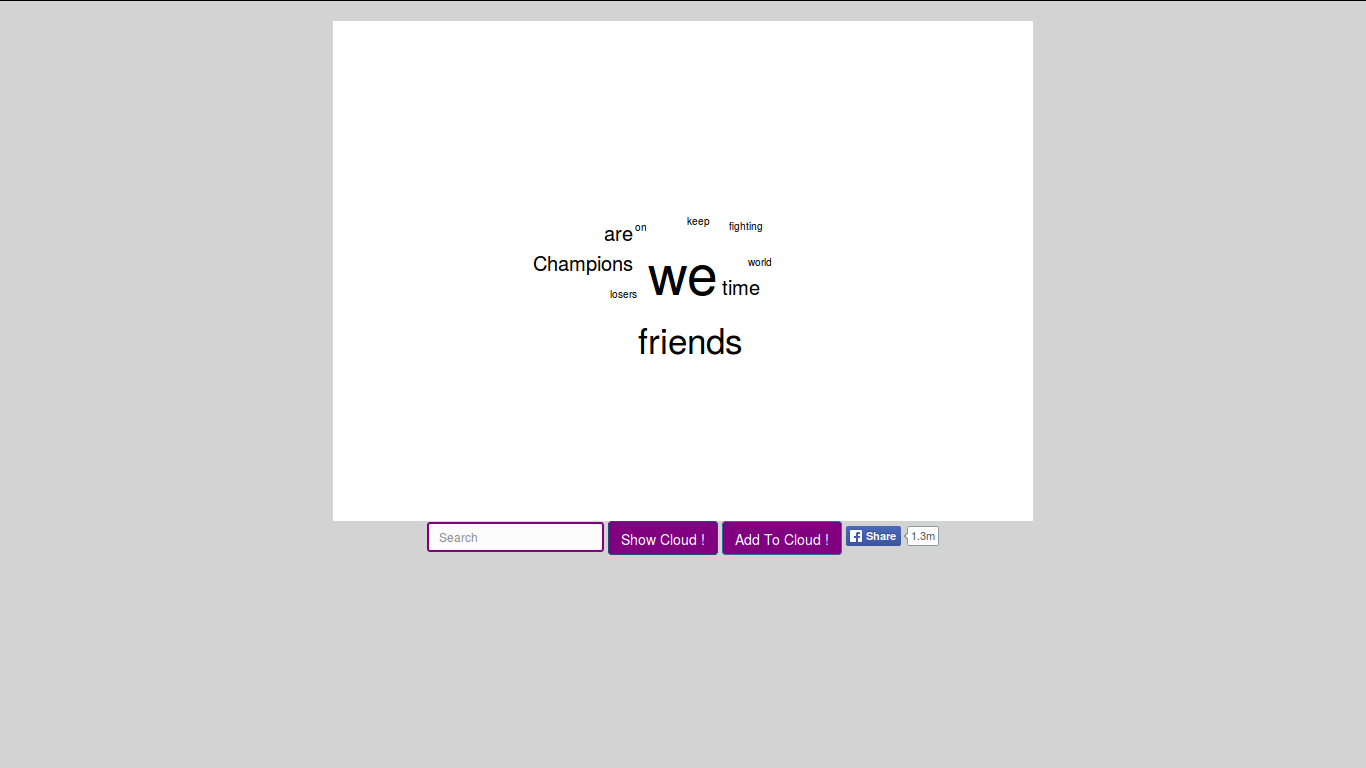
\includegraphics{Homepage.png}
\caption{Screenshot of the Homepage}
\end{figure}

\begin{figure}[htbp]
\centering
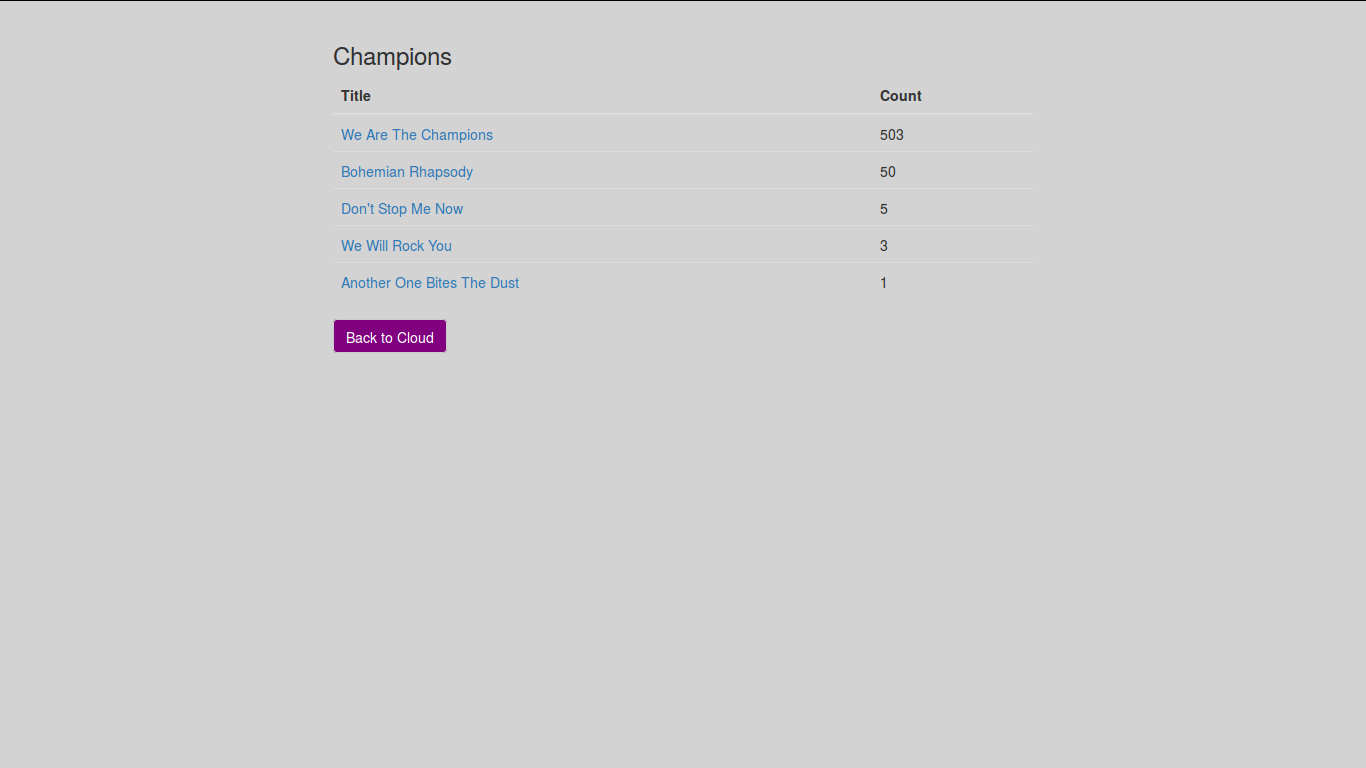
\includegraphics{SongsList.png}
\caption{Screenshot of the Songs List}
\end{figure}

\begin{figure}[htbp]
\centering
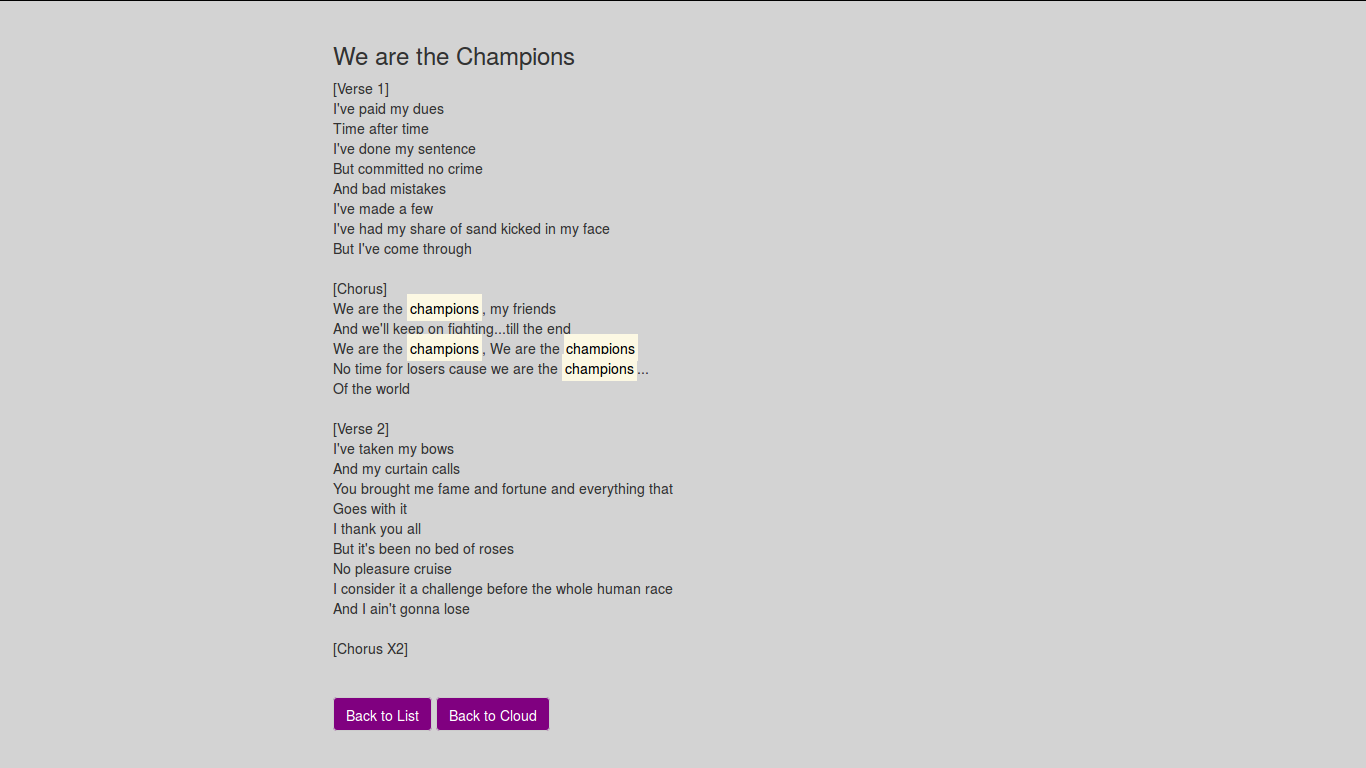
\includegraphics{SongPage.png}
\caption{Screenshot of the Lyrics Page}
\end{figure}

\end{document}
